\appendix

\chapter{Tecnologie Utilizzate} \label{appendix:a}

\section{Angular 8} \label{appendix:angular}
Angular è un framework di progettazione di applicazioni e una piattaforma di sviluppo per la creazione di app a pagina singola efficienti e sofisticate, utilizzando come linguaggi HTML, CSS e TypeScript. 

TypeScript è un linguaggio di programmazione open-source, sviluppato e mantenuto da Microsoft. È un soprainsieme di JavaScript (JS) a livello sintattico, con la differenza che è possibile utilizzare la tipizzazione statica per i dati.

Le funzionalità centrali e opzionali vengono implementate come set di librerie TypeScript, che possono essere importate nel progetto che si vuole creare. L'architettura di un'applicazione Angular, si basa su quattro concetti fondamentali, descritti di seguito.

\subsection{Modulo}
Un NgModule fornisce un contesto di compilazione per un insieme di componenti dedicato a un determinato dominio dell'applicazione, un workflow oppure un insieme di funzionalità strettamente correlate. Un NgModule può associare i suoi componenti al codice correlato, come i servizi, per formare delle unità funzionali. Un'applicazione Angular ha almeno un modulo radice, il quale è indispensabile per il suo avvio, e poi possiede altri diversi moduli ognuno con il proprio contesto.

\subsection{Componente}    
Ogni applicazione Angular ha almeno un componente, quello radice, che collega una gerarchia di componenti con il DOM (\textit{Document Object Model}) della pagina. Ciascun componente definisce una classe che contiene dati e logica dell'applicazione ed è associato a un modello HTML (e CSS) che definisce il livello di vista da visualizzare in un ambiente target, solitamente un browser web.
    
\subsection{Service e dependency injection}
Per i dati o la logica non associati ad una vista specifica e che si desidera condividere tra i componenti, si crea una classe service. Tali servizi possono essere iniettati all'interno dei componenti desiderati mediante il concetto di \textit{dependency injection}, il quale consente di mantenere snelle ed efficienti le classi dei componenti e dunque rendendo il codice modulare, riutilizzabile e performante.

\subsection{Routing}    
Il modulo router di Angular fornisce un servizio che consente di definire un percorso di navigazione tra i diversi stati dell'applicazione e visualizzarne le gerarchie. È modellato sulle convenzioni di navigazione del browser classiche, ossia l'inserimento di una URL nella barra degli indirizzi, click a collegamenti nella pagina, click sulle icone "indietro" e "avanti" del browser. Sostanzialmente il router esegue il mapping di percorsi simili ad una URL sulle viste (componenti), anziché direttamente sulle pagine. Quando un utente esegue un'azione, ad esempio facendo click su un collegamento, che carica una nuova pagina nel browser, il router intercetta il comportamento del browser e mostra o nasconde le gerarchie di viste.\\
Per definire le regole di navigazione, è sufficiente associare i percorsi di navigazione ai vari componenti. Un percorso utilizza una sintassi simile a un URL. È quindi possibile applicare la logica del programma per scegliere quali viste mostrare o nascondere, in risposta all'input dell'utente e alle proprie regole di accesso.

\section{Spring Framework} \label{appendix:spring}
Spring Framework fornisce un modello di programmazione e configurazione completo per le moderne applicazioni enterprise basate su Java, su qualsiasi tipo di piattaforma di distribuzione.

Un elemento chiave di Spring è il supporto infrastrutturale a livello di applicazione: Spring si concentra sulla gestione dell'infrastruttura delle applicazioni enterprise, in tal modo è possibile concentrarsi sulla logica di business sul livello applicazione, senza inutili legami con specifici ambienti di distribuzione.

\subsection{Caratteristiche}
Le principali caratteristiche di tale framework sono le seguenti:
\begin{itemize}
    \item Spring consente di sviluppare applicazioni enterprise utilizzando i cosiddetti POJO (\textit{Plain Old Java Object}). Il cui ulteriore vantaggio è che non è necessario un contenitore EJB (\textit{Enterprise Java Bean}) come un application server, ma si ha la possibilità di utilizzare solo un contenitore servlet robusto come Tomcat o altri prodotti simili commerciali.
    \item Spring è organizzato in moduli. Anche se il numero di pacchetti e classi è notevole, è sufficiente preoccuparsi di quelli necessari per l'esecuzione dell'applicazione.
    \item Si integra facilmente con framework già esistenti.
    \item Gestione centralizzata delle eccezioni. Spring fornisce un'API conveniente per tradurre eccezioni specifiche per la tecnologia (generate ad esempio da JDBC, Hibernate o JDO) in eccezioni coerenti e non controllate.
    \item Dimensioni ridotte.
    \item Sfrutta il concetto di \textit{dependency injection} e \textit{Inversion of Control}.
\end{itemize}

\section{Hibernate Framework} \label{appendix:hibernate}
Hibernate è un framework Java che agevola lo sviluppo dell'applicazione per quanto riguarda l'interazione con il database. È uno strumento per l'ORM (Object Relational Mapping), open source e di dimensioni ridotte. Esso implementa le specifiche di JPA (Java Persistence API), una libreria Java per la persistenza dei dati.

\subsection{Object Relational Mapping}
Un'ORM è uno strumento che semplifica la creazione, la manipolazione dei dati e l'accesso ad essi. È una tecnica di programmazione utile per mappare gli oggetti di un linguaggio di programmazione come Java, nei dati memorizzati all'interno di tabelle di una base dati relazionale.

\begin{figure}[H]
	\centering
	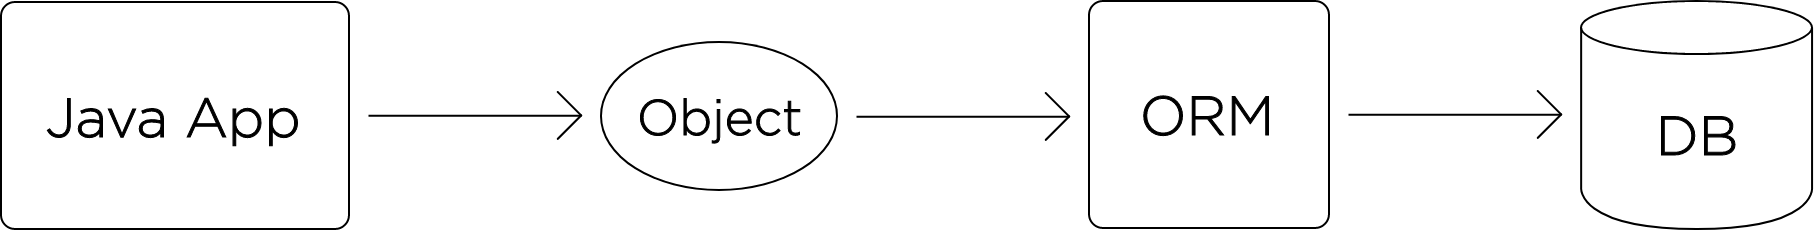
\includegraphics[width=.6\linewidth]{orm.png}
	\caption{Schema di alto livello di un'applicazione che sfrutta un ORM per l'interazione con un database relazionale.}	
	\label{fig:orm}
\end{figure}

Nel caso di Hibernate, quindi dell'utilizzo del linguaggio Java, viene utilizzato la JDBC (\textit{Java Database Connectivity}) API per permettere l'interazione con la base dati.

\subsection{Architettura del framework}
L'architettura di Hibernate coinvolge diversi tipi di oggetti, quali un oggetto di persistenza (da memorizzare), session factory, transaction factory, connection factory, session, transaction, ecc.\\ 
In generale possiamo categorizzarla in quattro livelli:
\begin{itemize}
    \item Applicazione Java.
    \item Framework Hibernate.
    \item Back-end API
    \item Base dati
\end{itemize}
Quanto appena detto, viene presentato in figura \ref{fig:hibernate}

\begin{figure}[H]
    \centering
	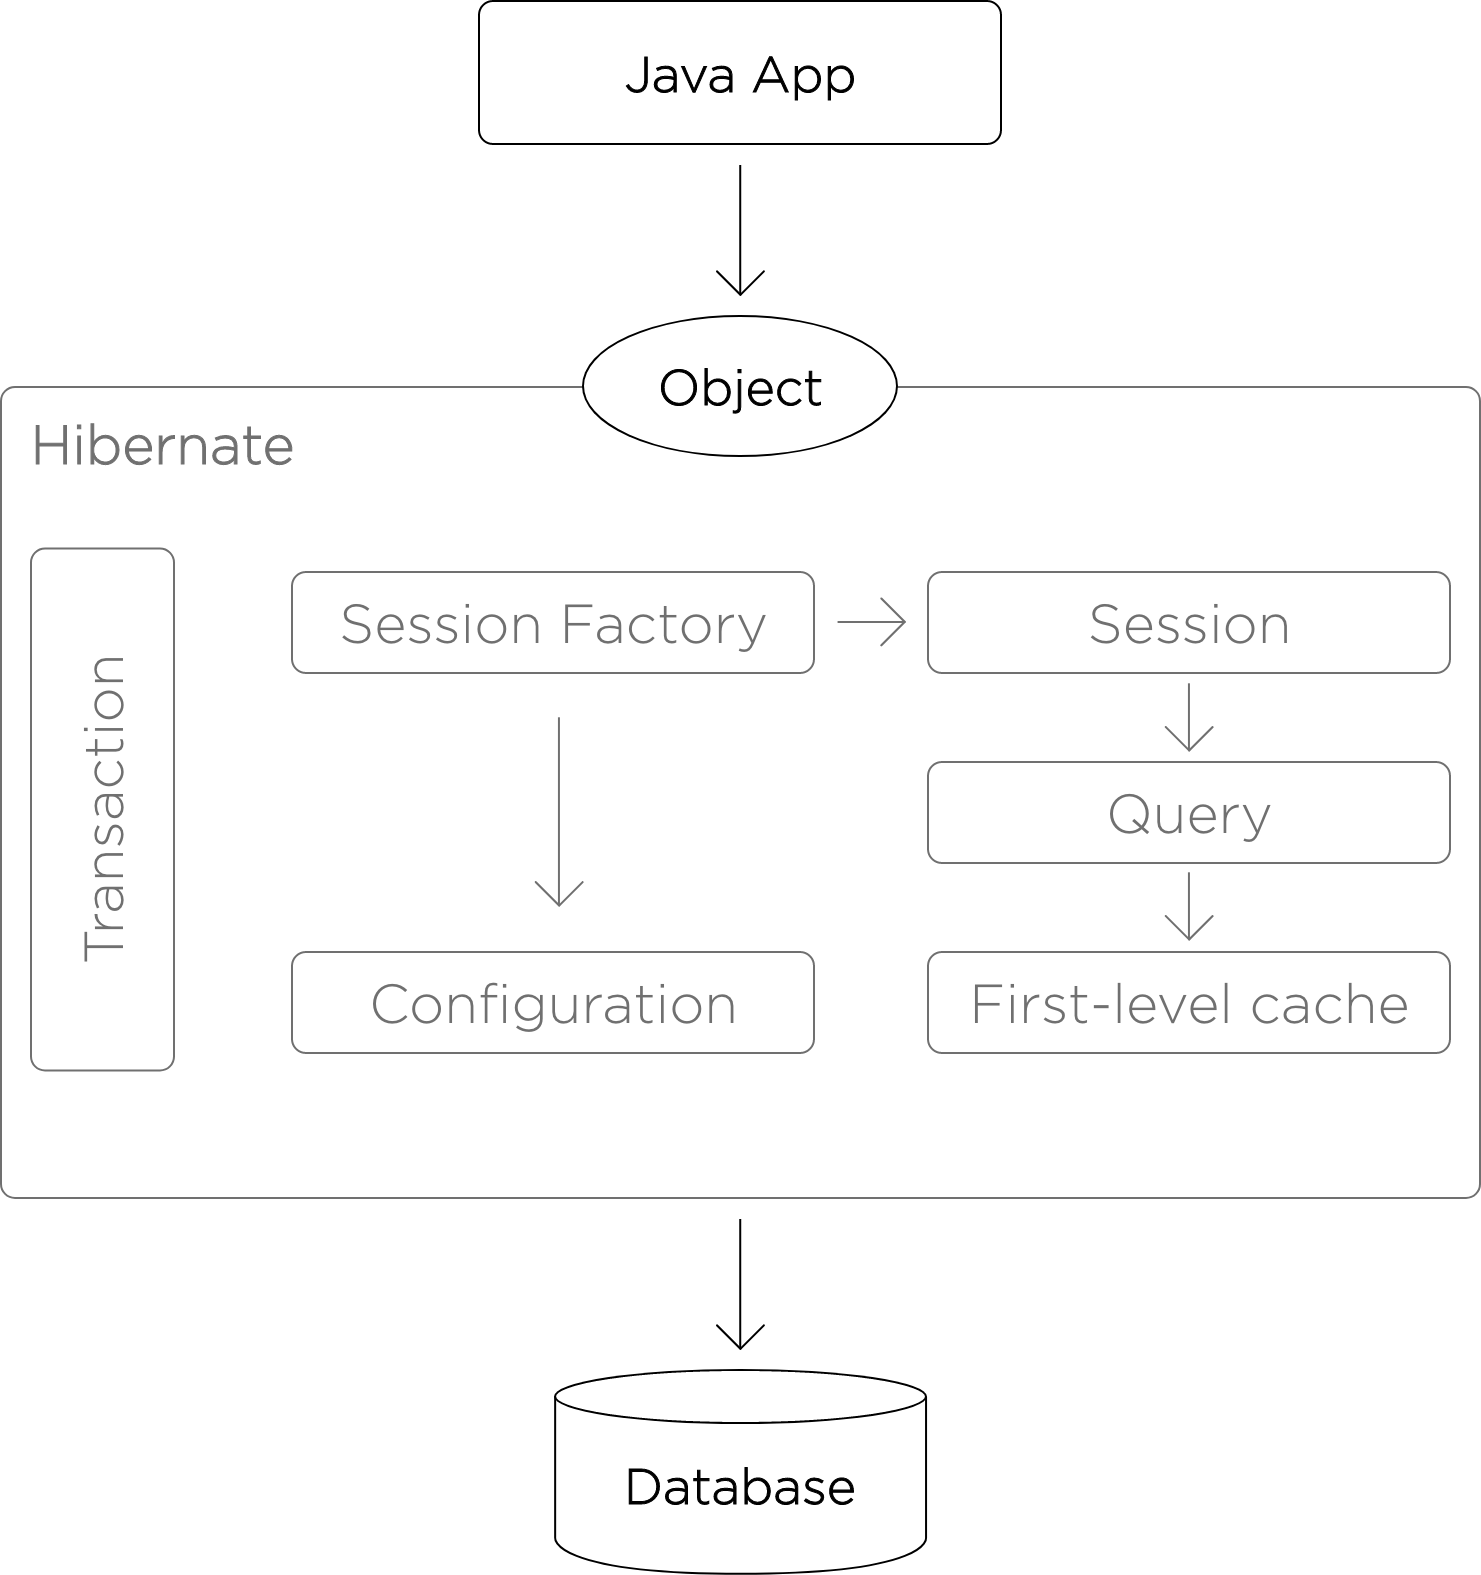
\includegraphics[width=.5\textwidth]{hibernate.png}
	\caption{Schema di alto livello di un'applicazione che adopera Hibernate per l'interazione con un database relazionale.}	
	\label{fig:hibernate}
\end{figure}